%\chapter{T-Ringの設計実装}
\chapter{設計と実装}
\begin{large}
\begin{quote}
本章では,T-Ringにおける詳細な設計,実装について解説する.
\end{quote}
\end{large}
\clearpage


\section{設計}
\subsection{システムアーキテクチャ}
%本節では,T-Ringシステムの設計について述べる.T-Ringを構成する保存ピアはネットワークモジュール,センサ情報管理モジュール,データ保存モジュール,データ取得モジュール,保存ピア発見モジュール,センサ管理モジュール,アプリケーションモジュールの7つのモジュールによって構成される.図\ref{fig:sysconf}がシステム構成図であり,各モジュール間でのデータの受け渡しが記述されている.
本節では,本システムのアーキテクチャ(図\ref{fig:system_architecture})を基に,
本システムの設計について述べ,
各モジュールについて詳しく説明する.


\begin{figure}[htbp]
 \begin{center}
  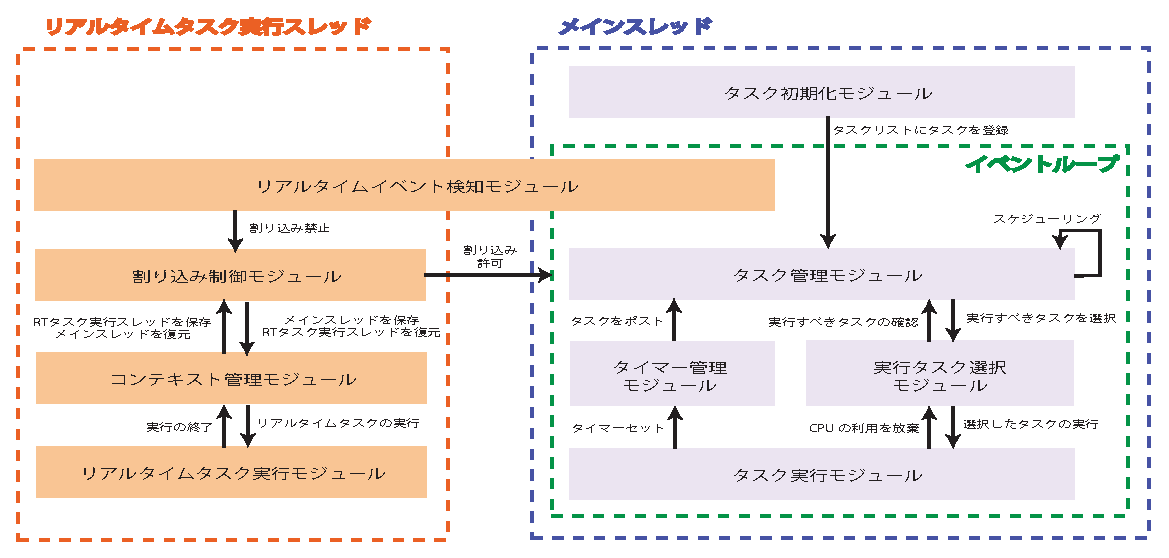
\includegraphics[width=150mm]{./images/system_architecture.eps}
 \end{center}
 \caption{システムアーキテクチャ}
 \label{fig:system_architecture}
\end{figure}


\subsubsection{タスク初期化モジュール}

\vspace{0.5em}タスク初期化モジュールは,アプリケーション開発者によって
初期化されたタスクをカーネルが保持するタスクリストに登録する.
本モジュールはアプリケーションがデプロイされたときにのみ実行され,
イベントループ内で実行されるモジュールと異なり,
複数回実行されることはない.



\subsubsection{タスク管理モジュール}

\vspace{0.5em}ここではタスク初期化モジュールにて,
登録されたタスクをタスクリストに登録し,
スケジューリングアルゴリズムに従って,
タイマー管理モジュールによってポストされるタスクを
実行される順番に並び替える.
実行タスク選択モジュールからの問い合わせがあった際には,
スケジューリング後の最も優先度の高いタスクのアドレスを渡す.



\subsubsection{実行タスク選択モジュール}

\vspace{0.5em}タスク実行モジュールにおいて,
実行中のタスクがCPUの利用を放棄した場合,
実行タスク選択モジュールにて,
次に実行するタスクを選択するために,
タスク管理モジュールに実行が最優先とされるタスクについて尋ねる.
タスク管理モジュールからの応答を待ち,
受け取ったタスクを次に実行するべく,
タスク実行モジュールへと引き渡す.



\subsubsection{タスク実行モジュール}

\vspace{0.5em}タスク実行モジュールでは,
タスク選択モジュールにて選択されたタスクを実行する.
実行中のタスクがCPUの利用を放棄した場合には,
次に実行するタイミングを決めるために,
タイマー管理モジュールに次の実行時間を知らせ,
タスク選択モジュールによって選ばれた
次に優先度の高いタスクを実行する.



\subsubsection{タイマー管理モジュール}

\vspace{0.5em}実行中のタスクが自ら実行を中断した場合,
タスク実行モジュールにて次に実行される時間が指定される.
タイマー管理モジュールでは,
タスク実行モジュールによってセットされたタイマーが発火した際には,
それに対応するタスクをポストするため,
タスク管理モジュールにタスクのポストを知らせる.


\subsubsection{リアルタイムイベント検知モジュール}

\vspace{0.5em}本システムの想定環境である,
環境モニタリングやターゲットトラッキングのようなアプリケーションでは,
イベントが発生した際に,他のどのタスクよりも優先してそのタスクの
実行を行う必要がある.
本モジュールでは,対象とするイベントが発生した場合に,
イベントループに割り込みをし,
他のスレッドにスイッチした際に割り込みが発生しないよう,
割り込み制御モジュールにて割り込みを禁止するシグナルの送信を依頼する.


\subsubsection{割り込み制御モジュール}

\vspace{0.5em}割り込み制御モジュールでは,
リアルタイムタスク実行中に他のタスクによる
割り込み処理が発生しないように制御を行う.
リアルタイム処理が終了した際には,
イベントループ実行中のメインスレッドにタスクの完了を知らせ,
割り込みを許可する.


\subsubsection{コンテキスト管理モジュール}

\vspace{0.5em}タスクの実行中に割り込みが発生した場合,
割り込みが発生しなかったときと同様の処理が行われなければならないため,
レジスタの値をスタックに退避させる.
それに対して,割り込み発生により実行されるタスクは,
以前の状態を取り戻すべく,スタックからコンテキストを復元する.
リアルタイムタスクの処理が完了し次第,
メインスレッドのコンテキストを復元し,
割り込み制御モジュールに割り込みを許可するように求める.



\subsubsection{リアルタイムタスク実行モジュール}

\vspace{0.5em}本モジュールは,コンテキスト管理モジュールでの
中断されたタスクの復元が完了し次第,
リアルタイム処理の必要なタスクの実行を行う.
タスクの実行が完了すると,
その旨をコンテキスト管理モジュールに伝え,
割り込み発生前の状態を復元する.






\subsection{タスクの状態遷移}



\subsection{スケジューリングアルゴリズム}






\section{実装}
\subsection{実装環境}
本システムはMicaZ上で実装した.
表\ref{tab:implementation_env}にMicaZ及びアプリケーション作成に
用いたコンパイラの詳細を示す.
開発言語としてC言語を使用した.


\begin{table}[htb]
  \centering
  \caption{実装環境}
  \begin{tabular}{|l||c|} \hline
  	項目	 & 環境 \\ \hline \hline
	CPU & Atmega128L \\ \hline
	Clock	& 7.37 MHz \\ \hline
	メモリ & 4 KB \\ \hline
	コンパイラ	& avr-gcc 4.5.3 \\ \hline
	無線チップ	& CC2420 \\ \hline
	オペレーティングシステム & Contiki 2.6 \\ \hline
	プラットフォーム & MicaZ \\ \hline
  \end{tabular}
  \label{tab:implementation_env}
\end{table}




\section{まとめ}
本章では,まず,ソフトウェアの構成について述べた,そして,個々のモジュールの細かな設計と実装について述べた.特に重要なアルゴリズムについては,各小節の末尾に実際のプログラムを掲載した.
